\section{Jamarske raziskave na Migovcu ali dvanajst bitk Monatipa}
Raziskovanje brezna \passage[cave]{Monatip} na severni strani \passage[Migovca]{Tolminskega} \passage{Migovca} je bilo že od začetka domena mlajših članov jamarske sekcije planinskega društva Tolmin. Po tem ko so Čadržni odkrili jamo za spodmolom je kmalu večini raziskovalcem postala neperspektivna. Največja zagovornika, da se jama konča ali se  poveže z breznom Planika sta kasneje postala najbolj zagnana raziskovalca jame. Sam sem jamo raziskoval dvanajstkrat in prav dvanajstič se je zgodil največji uspeh, povezava s sistemom. Teh dvanajst akcij me je spominjalo na prav toliko soških bitk prve svetovne vojne. 

\paragraph{Na prvo bitko} me je povabil Kletnik mlajši leta 2007. Bila sva sama. Kletnik je bil takrat najbolj  zagnan član. Škoda da le enkrat. Oba sva upala na veliko povezavo te jame z sistemom. Po zemljevidu ni manjkalo prav veliko do tega predvidevanja. Na koncu \passage[cave]{Monatip}a sta bile dve uganki, ki sva jih takrat razreševala. Prvo je bilo okno v kaminu. Preplezal sem do njega a zaman, nadaljevanje se je ustavilo. V drugo smer v globino se je odpiral meander v katerem že Fratnik ni dobil nadaljevanja. Kletnik se je z vso močjo stlačil  v ožino. Nazaj se je vrnil s prebito ustnico in okrvavljen povedal, da boj še ni končan. Navdušen je povedal, da se  jama  nadaljuje. Že naslednjega dne se je Izi z Čadržni vrnil do tega mesta. Spustili so se še v neznano brezno in kmalu prišli v \passage{Primadono}. 

\paragraph{Drugi poizkus} se je zgodil šele leta 2009. Ker je bila povezava s Primadono že uspela je bila na vrsti povezava z glavnim sistemom jam na \passage{Migovcu}. To bi bilo možno po neznanem in ogromnem kaminu na koncu jame, kjer se cepi pot za meander v \passage{Primadono}. Poklical sem še prijatelja Matjaža iz Kopra, zraven pa so bili še: Karin, Ana in Erik. Matjaž je preplezal polovico kamina. Ime smo mu dali \passage{Planika}.

\paragraph{Tretji poizkus} in zopet sta minili dve dolgi leti. Na sestanku je bilo dogovorjeno, da jama zagotovo ne bo prišla v sistem in naj se jo razopremi. Nad to odločitvijo sem bil razočaran. Leta 2012 sem bil v jami z Rokom. V najbolj nemogočih razmerah po obilnem deževju sva se močila po jami. Ni bilo veliko upanja in tudi poizkus preplezati kamin do konca je še visel na nitki. Toda uspelo mi je priplezati na vrh kamina in z Rokom sva videla, da se jama še ne zapre. Izgledalo je še kar vzpodbudno in jamo nisva razopremljala. 

\paragraph{Četrti poizkus} istega leta sem z Tjašo in Nejcem podal v \passage[cave]{Monatip}a. Še vedno nismo bili prepričani ali gre jama naprej. V podoru na vrhu nekega novega kamina smo naleteli na močan prepih. Po sto metrih horizontalnega rova smo se oddahnili. Jama je šibala naprej. 

\paragraph{Peti poizkus} Ista ekipa okrepljena še z Maffijem je z velikim navdihom šla ponovno k skrivnostni jami. Nekje v mislih je še vedno oznanjala velika povezava v celotni sistem jam na Migovcu in s tem tudi primat najdaljše jame v Sloveniji. Le ta se je zgodila  poleti. \passage[cave]{Monatip} je nekako tudi bil uključen v to tekmo a zaenkrat še brez uspeha. Tako brez obremenitve smo se podali po ozkih rovih in prišli do neznanega brezna.  Spustili smo se 40 m v globino. Sledil je še krajši rov ter kamin. Vse se je tu zaprlo. Po meritveh je od tu do sistema še okoli 100 m. Nov del z breznom smo poimenovali To ni naš problem. 

\paragraph{Šesti poizkus} 2013. Udeležili smo se ga: Čibej, Rile, Fratnik, Maffi in Tjaša. Treba je bilo poiskati novo pot. Tjaša je nad breznom To ni naš problem splezala 8m visoko do manjšega okna. Zopet se je odprla ozka horizontalna galerija, podobna tisti iz katere smo prišli. Prepih je spet nakazoval pot naprej in kmalu je sledilo novo 30m brezno. Krstili smo jo za Luzerja. Pod njim se odpre več rovov. Nismo jih raziskali do konca. Brez dvoma pa je kazalo, da se bo jama povezala v nekaj večjega. Navdušenje je v trenutku še bolj naraslo, ko je Fratnik na tleh dobil fix. Hitro pa se je izkazalo, da ne smemo prehitevati misli. Na pasu sem preštel  fixe  in opazil, da  mi je eden »odletel«... 

\paragraph{Sedmi poizkus} 2013 Tjaša, Maffi, Erik, Rile, fratnik, Zec in Jarc. Zadnja dva se nista mogla prebiti za ožine. Brez niju smo nadaljevali raziskave pod Luzerjem. Geološko novejši rov je vodil v notranjost \passage{Migovca}. Odprla se je pravcata galerija v kateri smo nabili prečko. Za njo smo prišli do globljega brezna nato še enega. Njuno globino smo ocenili na 50m. Po 30 m nam je zmanjkalo vrvi. Na polici kjer smo se ustavili so bili po stenah čudni izrastki. Te tvorbe so nas spominjale na telovadce in brezno je dobilo ime \passage{Telovadci}.

\paragraph{Osmi poizkus} 2013. Fratnik, Izi, Nejc, Tetley in Oly. Na \passage{Migovcu} je potekal raziskovalni tabor. Naval je bil velik. Prvič se nisem udeležil akcije v \passage[cave]{Monatip}a. Vesel sem bil, da jim še ni uspelo priti v sistem. Malo kasneje v juliju sem se pridrižil Fratniku, Maffiju in Eriku iskati pravo nadaljevanje s prepihom.  V galeriji pod Luzerjem smo se spustili v 50m brezno  katerega dno je bilo zabasano s podornim skalovjem. Preizkovali smo tudi ta labirint a se vse konča s slepim breznom ali krajšim kaminom. Tedenski napadi v jami nepojenjajo. Še vedno v času angleško-tolminske odprave poteka nova akcija v sestavi:  Fratnik, Clear, Tetly, Maffi, Nejc...poizkušajo na vsak način poizkati povezavo. Razdelili so se v dve skupini. Fratnikova je širila ožino v meandru na najgloblji točki v jami. Maffi in Nejc pa sta plezala prečko nad Luzerjem. Vse brez obetavnih nadaljevanj. 

\paragraph{Deveti poizkus} V jesenskem zatišju sva se z Žetkom in najinima familjema pojavila na \passage{Kal}u. Šla sva v \passage[cave]{Monatip}a plezat prečko, ki sta jo zadnjič začela Maffi in Nejc. Zabil sem tri fikse kot sta rekla. Toda po tem nisem bil iz prečke v rovu,  temveč padel v praznino. Po šoku in odrgninah sem poizkušal še en krat, zabil še dva fiksa in le prišel do police. Od tu sem nadeljeval do novega kamina in brezna, ki se poveže z Luzerjem, torej nič novega. 

\paragraph{Deseti poizkus} 2015. Vsa potencijalna nadaljevanja so se končala. Kazalo je, da se jama zares ustavlja. Po drugi strani in teoriji to skoraj ni bilo mogoče, saj je \passage{Migovec} ves preluknjan. Zopet smo preizkusili srečo: Rile, Fratnik, Maffi in prvič Truš. Nekaj časa smo raziskovali v dvojicah pa nobeni ni uspelo narediti načrtovanega dela. Ponovno smo se združili in Fratnik nas je popeljal do brezna blizu Telovadcov, kjer naj bi na prejšnji akciji opazil neko okno. Malo se nam je mudilo zato smo se hitro spustili v brezno in skozi okno zanihali v ozko galerijo. Že sem mislil, da spet ne bo nič, ko se Maffi zasmeje in pove, da gre jama ptav tu naprej. 

\paragraph{Enajsti poizkus} Čez en mesec smo bili spet na \passage{Migovcu}. V akciji so sodelovali: Zec, Fratnik, Truš, Rile, ki pa sem se zaradi bolezni obležal na \passage{Kalu}. Novice iz jame so bile zelo spodbudne in ekipa zadovoljna. Naleteli so na precej prostorno galerijo, sledili so ji vsaj sto metrov do velikega brezna. Nova galerija poteka vzporedno z galerijo Hot line v sistemu. Povezava je res že zelo blizu. 

\paragraph{Dvanajsta bitka} 
Po vojaško, zadetek v polno se je zgodil: 24. Oktobra 2015. Zgodovinski dan se je pričel tako, da sem z Izijem in Fratnikom prišel do vhoda \passage[cave]{Monatip}a in se po desetih urah jame pojavil na vzhodni strani Migovca pred jamo M-16. Povezali smo vse jame v celotni sistem, ki je bil takrat dolg že več kot 35 kilometrov. 

\section{Speleological exploration on Migovec --- two months of battle}

In the beginning, the exploration of \passage[cave]{Monatip} cave on the slopes of \passage{Tolminski Migovec} was the onus of the younger members of the JSPDT. After the original discoverers explored the cave to its deepest point, expeditions soon became sporadic. The main advocate for the cave's potential connection with \passage{Planika Jama} later became one fo the most active explorers; I explored this cave myself twelve times, and the twelth round was the most successful, ending  with a connection to \passage{Sistem Migovec}. \bignote{These twelve assaults reminded me of the equally many battles of the First World War}.

\paragraph{The first battle}
Kletnik invited me early on in 2007. We were alone. Fratnik was then president and also the most active member, so it's a shame we only went together once. We both were hoping for a connection between \passage{Monatip} and the \passage{Sistem}, but there was not much to be expected from the map. At the end of the cave were two puzzles, which we both resolved on that visit. First was a window in the main aven of the \passage{Big Chamber}. I climbed to it, but this was in vain, as it died very soon. The second was a newly found meander, but Fratnik did not manage to continue through. He struggled with all his might, but turned back with a pierced and blood lip, saying that it was not over yet, and that, excitingly the cave continued. The very next day, he and Izi returned to this place. They descended an undiscovered pitch and soon entered \passage{Primadona}. 

\paragraph{The second battle} It did not take place until 2009. Since the cave had been successfully connected to \passage{Primadona}, the purported link to the \passage{Sistem} was, in turn, investigated. There was a possibility that it could start from a huge, unclimbed aven, towards the end of the cave, where the rift to \passage{Primadona} peeled off. I also invited my friend Matjaž from Koper, along with Karin, Ana, and Erik. Matjaž climbed halfway up the aven. We named it \passage{Planika}.


\paragraph {The third battle} Two long years ago.\sidenote{2011?}. At a club general meeting, it was decided that the cave would definitely not connect with the \passage{Sistem}.  I was disappointed with this decision. In 2012, I was in the cave with Rok.  In the most impossible conditions, after heavy rain we crawled through \passage[cave]{Monatip}. There was little hope, and even trying to climb the aven hung in the balance, but she managed to reach the top, and with Rok, we saw that the cave had not yet closed down. It looked very encouraging so we left the tackle on the pitch.


 \paragraph {The fourth battle} I went to \passage[cave]{Monatip} with Tia{\v{s}}a. and Nejc in that same year. We were still unsure whether the pitch would continue. \bignote{In the alcove at the top of the new aven, we found a howling draught, and after a hundred metres of horizontal passage we relaxed: the cave goes on}.


\paragraph{The fifth battle}  The same team, reinforced by Maffi, went back to the mysterious passage. At the back of our minds, we pictured the great connection of the entire cave system under \passage{Migovec}, cementing its primacy as the longest cave in Slovenia. It happened during that summer. \passage{Monatip} was also involved in the effort, but remained resolutely separate. Without much effort we passage through tight crawls to an undescended pitch, and abseiled down 40m. There was a short gallery and an aven. All dead around there. After the surveying, we measured about 100m distance from here to the system. We named the new passage and the pitch `This is not our problem' \sidenote{To ni naš problem}

\paragraph {The sixth battle} 2013. The following were in attendance: Čibej, Rile, Fratnik, Maffi and Tjaša. It was necessary to find a new way on. Tjaša climbed 8m above the \passage{To ni naš problem} pitch to a small window. Again, there was a horizontal gallery, very similar to the one we had come from. Tjaša indicated the way on and soon,we came to a 30m pitch. We christened it `\passage{Loozer}' for her. There were several rifts leading off at the bottom, which we did not all investigate to the bitter end. It appeared certain that the cave would soon connect into something bigger. The excitement grew momentarily as Fratnik put a bolt in the wall, but it quickly turned out that we should not get ahead of ourselves. On the traverse line, I counted the number of spitz, and noticed that one of them had `flown off'...

\paragraph{The seventh battle} 2013. The team: Tjaša, Maffi, Erik, Rile, fratnik, Zec and Jarc. The last two could not fit through the squeezes, so we continued exploration underneath \passage{Loozer} without them. This newer (geologically speaking) gallery led towards the heart of \passage{Migovec} and opened up at a junction with another gallery to the right. We descended a pitch and then another. Their depth was estimate ad 50m. After 30m, we ran out of ropes, and stopping on the shelf we noticed strange protrusions on the walls. These reminded us of gymnasts and the pitch was named `\passage{Telovadci}'.

\paragraph{The eighth battle} Fratnik, Izi, Nejc, Tetly and Oly \sidenote{Oliver Myerscough}. The summer expedition on \passage{Migovec} was up and running. The endeavour was substantial and for the first time I was not in the thick of it in \passage[cave]{Monatip}, but I was glad that they did not manage to find the way into the system without me. A little later in July, I joined Fratnik, Maffi and Erik to look for a continuation, using the cave draft. In the gallery below the \passage{Loozer} we descended into a 50m pitch, at the bottom of which there was scree-filled boulder choke. \bignote{We also tried to break through this labyrinth, but it all ended with a blind pit or small aven. The weekly assaults on this part of the cave did not relent}. At the time of the English exodus from Tolmin, a new action was planned, with the following team: Fratnik, Clare, Tetley, Maffi, Nejc... try to make a connection in any way. They were divided into two groups. Fratnik \textit{spread the strait in the meander} at the deepest point in the cave. Maffi and Nejc climbed to traverse over Loozer. All ended without promising leads.

\paragraph{The ninth battle} In the autumn silence, we appeared with \passage{Kal}y and our families at \passage{Kal}. We went to the \passage[cave]{Monatip} climbing a new pitch, an initiative launched by Maffi and Nejc. I forgot three bolts as I said. But after that, I was not clipped in from a \textit{bar in a trench}, but fell into the void. After the shock and some abrasions I tried my luck another time, drilled in two more bolts and only came to a shelf. From this position, I could see an aven and a pitch that connected back with \passage{Loozer}, so nothing gained.

\paragraph {The tenth battle} 2015. All potential leads have ended. It seemed that the cave really stopped. Of course, we knew this is practically impossible, since \passage{Migovec} is entirely hollow! Again, we tried our luck: Rile, Fratnik, Maffi and Truce for the first time. We pushed for a couple of times in pairs but nobody managed to find the connection. We reunited again and Fratnik led us to the abyss near \passage{Telovadci}, where he had noticed a window on the previous campaign. We were very worried, so we quickly went down into the abyss and rolled out of the window into a narrow gallery. I thought that there would be nothing again, but I found Maffi laughing and pointing out the ongoing shafts.

\paragraph {The eleventh battle} One month later, we were again on \passage{Migovec}. The campaign included: Zec, Fratnik, Truš, Rile, who, however, had to wait at \passage{Kalu} due to illness. News from the cave were very encouraging and the team satisfied. They encountered a rather spacious gallery, which they followed for at least a hundred meters to a large abyss. The new gallery runs parallel to the Hot Line gallery in the system. The connection is really very close.


\section{Dvanajsta bitka - The Twelfth Battle}

\margininbox{Monatip}{
     \begin{citemize}
    \item Andrej Fratnik
    \item Iztok Mozir
    \item Dejan Ristić
    \end{citemize}}{\explo}
Zadetek v polno se je zgodil 24. oktobra 2015 Čudež pod Migovcem, skoraj po vojaško. Okoli 17.00 popoldne se je zgodil zgodovinski dan. Skupaj z Fratnikom in Izijem smo iz \passage[cave]{Monatip}a skozi ožino prišli v poznane dele, galerijo v jami \passage{M18} in povezali vse tri sisteme na Migovcu. Nov sistem je tako dolg več kot 35 km. Moj dvanajsti obisk te jame je kot 12 soških bitk. Sicer so se zgodile točno pred sto leti, zanimivo je pa da se je zadnja imenovana »čudežna« bitka dogajala ravno oktobra isti mesec kot naša v jamo. 

  Vse se je dogajalo tako: V četrtek 22. oktobra me je poklical Izi, če grem v \passage{Monatipa} in na \passage{Kal} kjer bodo praznovali rojstni dan. Skromno pove, da je brez opreme in naj mu jo bo priskrbel Fratnik. Med drugim doda, da povezave ne bo in da če imam delo naj raje ostanem doma. Še bo čas, me tolaži. Hudiča, zopet se vse križa. Delo z novo hišo, Sandrina operacija, zopet in otroci počitnice. Pa še jama. Sem mislil, da gremo kasneje, zdaj pa mi od vsega kar gori glava. Neznansko me vleče gor. Čutim, da bo povezava glede na pretekle dogodke vsak čas padla in zato sem kot na trnih. Prespim še eno noč in poizkušam uskladiti vse zadeve. Naporni petek se začne zjutraj s službo, popoldne z gradnjo, zvečer še nabava gradbenega materiala za hišo in nato končno pakiranje za v jamo. Sandri povem še tisto zarečeno trditev, da če bo povezava sem končal z jamami.  Ob desetih zvečer zapustim dom in se sam odpravim skozi gozd. Zopet ista pesem. Sam z vsemogočimi skrivnostnimi mislimi. Kot velikokrat tiste o življenju in smrti. Tišina in redki šumi so moji spremljevalci. Da mi v tej temačni samoti ne bi bilo tesno si nekaj naglas pojem. Lepo je pa gledati v skoraj okroglo Luno, ki me ves čas spremlja ravno nad obronki gozda. Na trenutke je tako svetlo, da ugasnem luč in že vstopim v polno kočo na \passage{Kalu}. 

  Sobotno jutro se prikaže v najlepši jesenski varianti. Širina obzorja plane v mojo dušo. Sončni žarki obsijejo ves prostor, razen meglenih dolin. Dan se je začel z neko posebno energijo. To se občuti tudi med planinci, ki hodijo mimo. Presenečen zagledam svojega bivšega motorističnega prijatelja. Spremenjen je v žensko z imenom Saša. Skupaj popijemo štamprle žganice, predsodki izginejo in vsak gre s svojo zgodbo k svojemu cilju naproti. 
  
\begin{figure*}[t!]
\checkoddpage \ifoddpage \forcerectofloat \else \forceversofloat \fi
\centering
\frame{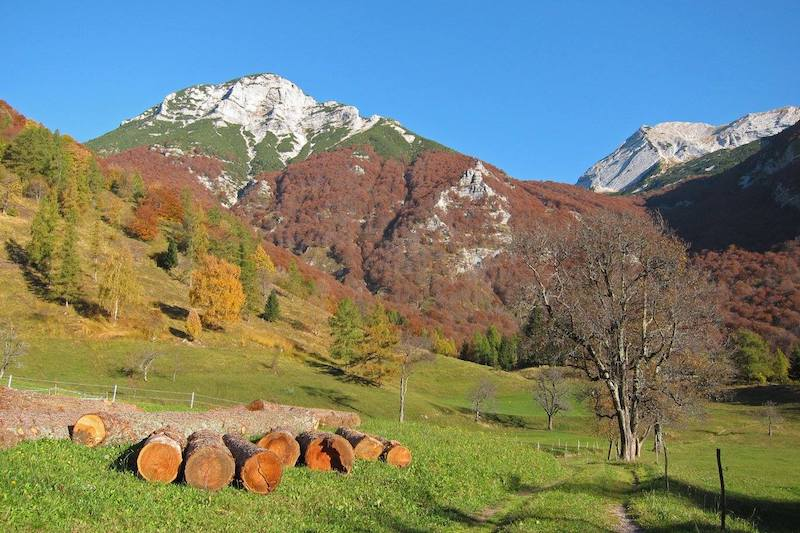
\includegraphics[width=\textwidth]{images/2015/rile-connection-2015/migovec_in_autumn.jpg}}
\caption{Tolminki \protect\passage{Migovec} in Autumn, before a major October `Super-Action' --- Jana Čarga }
\label{migovec in autumn}
\end{figure*}

  Opreme za v jamo nimamo veliko. Fratnik ima malo mašino, štrik pa je v jami. Merilni komplet je pri meni. V koči za vsak slučaj vzamem še nekaj ploščic in karabinov. Večina ostalega moštva se raje odloči za užitke na površju. Čez vhod zopet prileti kamenje. Izi je »full« žejen in mi popije skoraj vso pijačo. Posledica pretekle noči ga bo spremljala skoraj celotno akcijo. Po jami se premikam zelo preudarno. Potrpežljivo čakam, da bi videl kraj kjer so zadnjič odnehali. Prijatelja sta hitrejša od mene in komaj jima sledim. Ne veseli me tako hitri tempo. Po samo dobrih stvareh želim danes zares uživati v jami in biti del nje. Vanjo smo vstopili ob 10  zjutraj in po dveh urah smo že pred velikim nepoznanim breznom v galeriji \passage{Vzporedni svet}. Opazujem po breznu navzdol. Vidim prav do dna tega okrog 60 m brezna. Iz moje ptičje perspektive se pogled ustavi na peščenem ravnem dnu. Bog ve kaj vse je še spodaj. Na nasprotni strani opazujem po odprtini o kateri je govoril Maffi, da je možno nadaljevanje. Tu v rovu sredi brezna opazujemo situacijo in Fratnik se prvi odloči za spust v neznano. Trideset metrov pod nami se vidi na desno ogromno razširitev v katero bo čez nekaj časa Fratnik zanihal. Z Izijem razrešujeva zavozlani štrik in ga dodajava v globino. Minute minevajo in Fratnik porabi zares veliko časa da zabije tri svedrovce. Zelo mi je mraz v prste. Iz rova se potegnem v sredino brezna in spet čakam. Zaradi mirovanja so moji prsti otrpli in boleči. Končno se Fratnik le zavihti v stransko razširitev in zabije svedrovec na najbolj neugodno mesto. To je ogromna skala stoječa prav na robu brezna. Giljotina. Fratnik jo krsti za Pojočo skalo. 

Če bi se premaknila in zgrmela bi nas potegnila v globino. Raje ne razmišljam o tem in se poizkušam čim prej skobacati iz brezna na začetek ogromnega novega sveta, ki ga ni videl še nihče pred nami. Naše razpoloženje je prav zaradi dimenzij tega prostora drugačno kot prej celo jamo in celo mesece prej. Odprlo se je zares nekaj velikega in zdi se kot bi bili na nekem križišču ali pa otoku brodolomcev. Neznansko nas vleče naprej. Ne vem kako bi to stanje zadovoljstva sploh opisal. Hodimo po ogromnem horizontalnem hodniku, kot bi se zmagovalci sprehajali na paradi. Opazujemo galerijo in padajo besede: »Lej to, lej to, uf, mater…« Naše poglede pritegnejo čudne tvorbe kapnikov in kamnov. Eni izmed kamnov so temnordeči, drugi pa že vlečejo na zeleno. Vsak vzame kakšen košček. Fratnik poda hipotezo, ki jo je nekje slišal, da so na teh kamnih bakterije, ki jejo to kamenje. In res so bile na teh skalah neke črne kolobarjaste tvorbe. Prikladno ime rov postane Kamnožer.  Sproščena pot se ne konča. Le kam vodi? Pomerim s kompasom smer. Galerija nas vodi še preveč po pravi smeri. Namesto v smeri 60 stopinj, ki bi nas pripeljala do brezna \passage{Mig Country} hodimo sedaj že skoraj proti severu. Pot poteka rahlo navzgor in prehodili smo že vsaj 200m. Vsi smo iz sebe. Po tolikih akcijah je to darilo. Kaj nas še čaka? Kako bo izgledala povezava se sprašujemo? Naposled se ustavimo pred podorom. Kupi oglatega kamenja so z leve strani zasuli skoraj ves rov. 


\begin{figure*}[t!]
\checkoddpage \ifoddpage \forcerectofloat \else \forceversofloat \fi
\centering
\frame{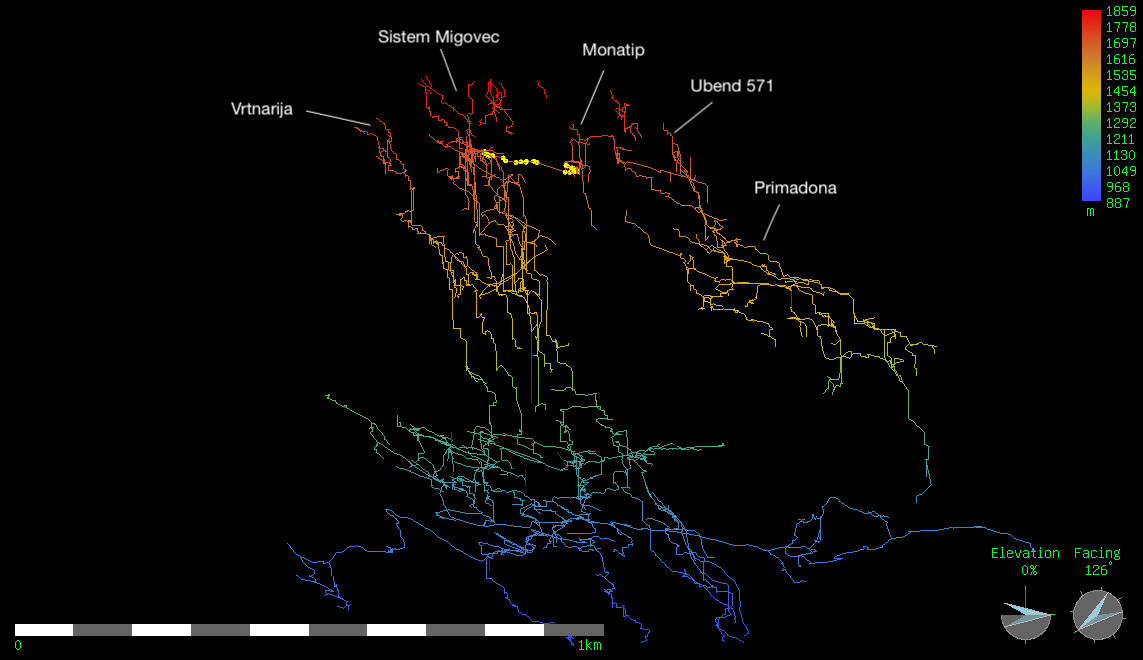
\includegraphics[width=\textwidth]{images/2015/rile-connection-2015/monatip connection.png}}
\caption{A highlight of the connection passages between \protect\passage{Sistem Migovec} and \protect\passage{Monatip}-\protect\passage{Primadona}-\protect\passage{Ubend 571}. --- produced on \emph{Aven} }
\label{migovec in autumn}
\end{figure*}


Med kamenjem in steno je ozek precej zasut prehod, skozi katerega se vidi temo. Povrhu pa še močno piha. Lotimo se odmetavanja kamenja. Menjujemo se v ožini. Delo postaja po določenem času vedno bolj neuspešno. Na Izija se kruši material in postaja že nevarno. Fratnik predlaga, da pridemo drugič z stvarmi za miniranje. Nič, čaka nas pripravljanje za povratek in merjenje. Čakam pred ožino. Nekaj mi ne da miru. Poizkušam še zadnjič odgrebsti nekaj kamenja. Zviz v ožino in kopljem. Nekaj časa kopljem in zazdi se mi, da pa bi najbolj suhi Izi že mogel skozi najožji del. Izi proba in uspeh je tu. Je že na drugi strani v majhni razširitvi. Sledi mu še Fratnik. Vprašam kako je? »Nova ožina« reče Fratnik. Nekaj časa prekladata kamenje in sliši se rušenje skal. Naposled še sam slečem pas in jima sledim. Medtem Fratnik že izgine po drugi dolgi ožini. Malo pred tem sta na steni te razširitve opazila piko podobno tisti, ki jo naredi karbidovka. Čakava in neko čudno vzburjenje narašča. Kmalu zaslišiva Fratnikove besede: »Pobje dans bo veselje, dans bomo odprli šampanc.« Na moment se mi vse oddahne. Preprosto, povezava! Leta pričakovanj so zdaj prinesla darilo. Ampak še vedno sem malo zmeden in ne verjamem sto procentno. Zopet Fratnik: »Tu je po tleh karbid in več pik po steni.«  Ironično dodam »Nismo še zmagali« in Fratniku odgovorim, da je zame dokaz samo fiksiran štrik, saj karbid lahko prinese voda iz višjih mest. Potem pa se Fratnika ne sliši več. 

Po trebuhu mu sledim še deset metrov in iz oklepa ožine prihajam v pokončno lego do tistih črni, sajastih pik. Resnično nekdo je tu že bil. Sledim vse bolj širokemu delu do prave galerije. Zasliši se Izija: »Tu je štrik. In tu je še eden. Rile, tu je tolk štrika kolkr ga hočeš.« Zares to je povezava. Sprva je še vse uganka v katerem delu jame smo. Pričakovali smo galerijo Hot line, pa ji to ni podobno. Očitno smo jo »preskočili«, šli nekje nad njo in prišli v manjšo galerijo, ki bi lahko bil \passage{NCB} tunel. Ko pridemo k ostankom  angleškega tabora dvomi izginejo.  Zagotovo smo prišli  v brezno \passage{M18}. Opazujemo okolico in se s spomini vračamo v leta, ko so tu raziskovali Angleži. Tudi Fratnik in Izi prepoznata te dele, ker sta tu že nekoč bila. Kakšen fantastičen občutek je tu sredi rova opazovat in z mislimi tavat po tem labirintu. Cilj je dosežen in neka velika sprostitev napolnjuje telo. Čeprav nismo na nobenem vrhu je ta točka vrhunec neke poti, podzemske poti. Spomnim se tudi na leto 1995, ko so tu Angleži dosegli višek svojih raziskav. Citirali so N. Castereta. »Do velikih stvari prideš po ozki poti.« Kar je \passage{M18} tudi bila. Jama ožin in strganih kombinezonov. Toda Angleži na koncu galerije niso prekopali vsega. Če bi jim uspelo, bi našli še večjo galerijo po kateri smo prišli danes mi. 
  Sklenemo vrniti se po plezalno opremo za ožine nato pa se po drugi strani in drugih jamah vrniti proti izhodu. 
\begin{figure*}[t!]
\checkoddpage \ifoddpage \forcerectofloat \else \forceversofloat \fi
\centering
\frame{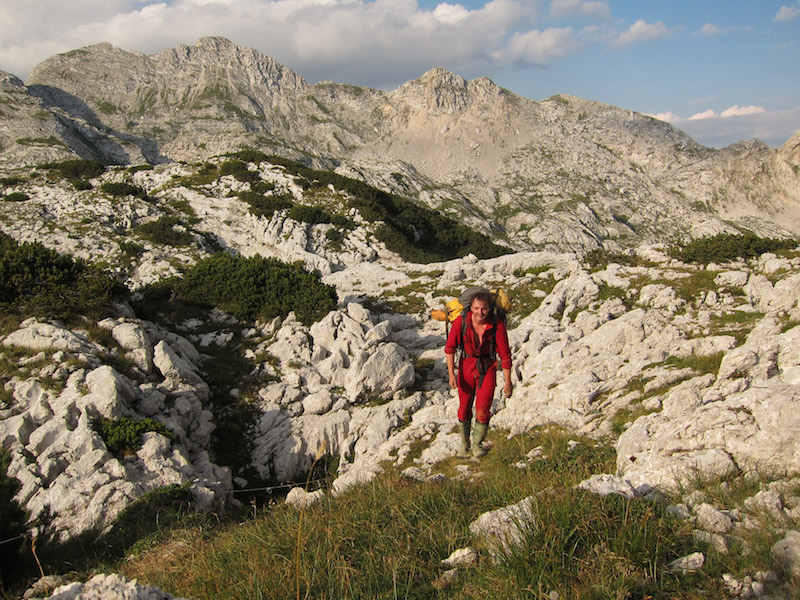
\includegraphics[width=\textwidth]{images/2015/rile-connection-2015/jana-plateau-surface.jpg}}
\caption{Jonathon Hardman trudging along with a heavy bag across the lunar landscape of the \passage{Migovec} Plateau--- Jana Čarga }
\label{mig surface jon hardman}
\end{figure*}

\begin{figure*}[t!]
\checkoddpage \ifoddpage \forcerectofloat \else \forceversofloat \fi
\centering
\frame{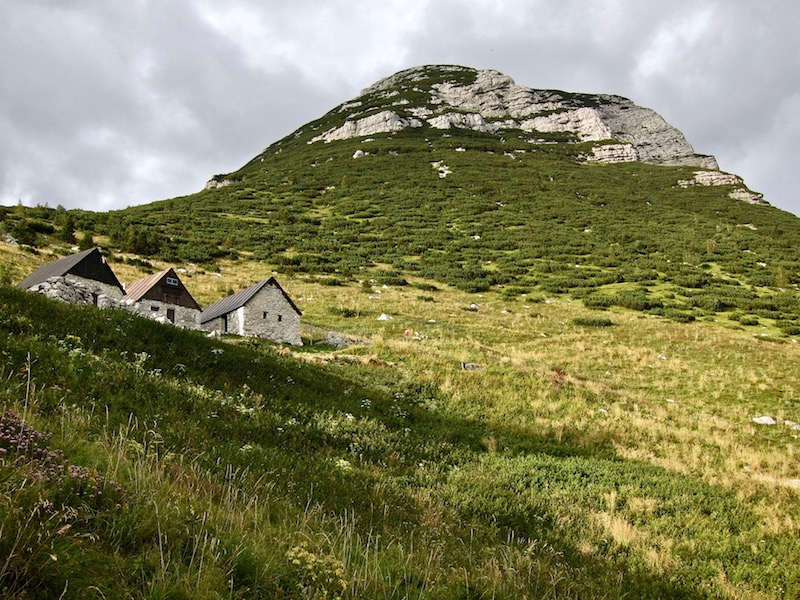
\includegraphics[width=\textwidth]{images/2015/rile-connection-2015/face_of_migovec__1_.jpg}}
\caption{The \protect\passage{Migovec} face, as seen from the switchback trail under \protect\passage{Planina Na Kalu}, the Shepherd's Hut--- Jana Čarga }
\label{migovec south face}
\end{figure*}

Naredili bomo krog pod zemljo. Merjenje opustimo za drugič, zmanjkalo nam bo časa. Ura je okoli 17.00 popoldne. Vse je OK. Le mene je strah, da zadnja brezna v M-16 niso opremljena. Vrnemo se nekaj deset metrov po galeriji nazaj in splezamo v ožino ter po trebuhu eden za drugim rijemo in se spuščamo do »Level 2« v sitemu Mig. Kot bi gledal iz avtobusa že znane postaje prihajajo iz noči: \passage{Titanik}, \passage{Mig Country}, \passage{Gladiatorska} prečka…V teh ogromnih sobanah preluknjanih z globokimi brezni smo le tema in mi. Ves čas se ob tem sprašujem, do kdaj bom še gledal to podzemlje? Še bolj kot to me znova mori paranoična misel, kaj, če je kdo v resnici pobral štrike iz vhoda Šestnajstke. To bi pomenilo, da se moramo ponovno vrniti skozi celo jamo…Ko sem končno pod vhodnim delom in zagledam štrik sem presrečen. Rešeni smo, prihaja drugi lahko rečem vhod ali izhod. Zdaj pa res med plezanjem sanjam in se spominjam čas pred davnimi 35. leti, ko sem kot mulc z Iliado in Zoranom tu nabiral prve jamarske izkušnje. Okoli 20 ure smo vsi trije pred vhodom. Zunaj je tema, nekaj snega in Luna. Zazremo se v zvezde. Kaj vse je nad nami? Po površju Migovca iz zahodne strani prečimo proti zahodni, do prehoda med Migovcem in Kukom kjer se moramo po ovčji stezi spustiti do vhoda \passage[cave]{Monatip}a. Tam nas čakajo ruksaki in iz svojega nam Fratnik ponudi pivo. Odrinemo na izhodišče na \passage{Kal}. Po juhi in pašti odrinem ponosno v dolino. Zraven pa me spet spremlja Luna. Zgodil se je zgodovinski dan in z jamarstvom lahko odneham.  
 
\name{Dejan Ristić}


\section{The Twelfth Battle}
\margininbox{Monatip}{
     \begin{citemize}
    \item Andrej Fratnik
    \item Iztok Mozir
    \item Dejan Ristić
    \end{citemize}}{\explo}

The miracle that took place underneath \passage{Migovec} on the 24th of October 2015 had almost a military feel. This was achieved at 17:00 in the afternoon on a historic day. Together with Andrej Fratnik and Izi, we went straight from \passage[cave]{Monatip} entrance to the galleries of M18 and connected the three systems of \passage{Migovec} making the new combined system more than 35km long. My twelfth visit to this cave echoed the Twelfth battle of the Soca. The latter happened exactly a century ago, but it is interesting to note that the aforementioned miracle `battle' occured this same month of October underneath \passage{Migovec}.   



Everything started like this: on Thursday 22th October I received a call from Izi, asking whether I'd like to go to \passage[cave]{Monatip} from \passage{Kal}, where they were celebrating a birthday. He adds modestly that Fratnik will provide the equipment. He also said that there probably wouldn't be a connection, that since I had a job, I might prefer to stay home. I had earned my comfort. Hell, once again my heart was conflicted. Working in the new house, Sandra operated again and kids' holidays. And the cave. I thought to go caving a little later, but the thought burned in my head. It was drawing me towards Mig. I felt that, thanks to recent efforts, the connection would be found in a matter of time, this was making me anxious. I spent one night trying to coordinate everything. A very busy Friday started with a job in the morning,  construction in the afternoon, ordering building supplies for the house in the evening, and finally the packing of caving equipment. Sandra will tell you of a heated argument: should I find the connection, I'd have to stop caving!  At 10'o clock in the evening, I left the house and entered the forest. \bignote{You know that song: lost in mysterious thoughts with the Almighty, often thoughts of life and death. Silence or soft murmurs are my only companions. This dark solitude could not quell my anxiety though.} The moon was almost full, watching me above the forested foothills. It was so light at times that I turned off my torch, until I reached a packed cottage at \passage{Kal}.

Saturday morning began coated in the most beautiful shades of Autumn. The width of the horizon engulfed my soul. The sun's rays painted the entire landscape in bright colours, except for the misty valleys. The day started with a unique energy, which was felt by some hikers walking past. I was surprised to find that he was looking for former biker friends. With him, a woman called Sasha. They were completely drunk, requested lots of Zganje and soon prejudices disappeared with each sharing their story and goals.

We do not take much equipment. Fratnik takes a tape-measure for the cave. The rest of the surveying kit is with me. I steal a few carabiners and bolts from the hut, just in case. The others prefer the surficial pleasures. We approach the cave entrance across the scree slope. Izi feels very thirsty, and I downed almost all our drinks. The consequences of the previous night would hound us throughout the entire campaign. We move cautiously across to the cave.  My friends are normally faster than me but today they barely keep up with me although I don't have a quick pace. We really enjoyed caving that day, being part of it. We entered \passage[cave]{Monatip} at 10 in the morning, and after two hours, we reach the `\passage[|see Vsporedni svet]{Parallel Gallery}', facing a big unfathomed abyss.

 I peer down it. \bignote{My light reaches all the way to the bottom of this 60m shaft}. From my vantage point, I can see sandy ledges on the bottom section. God knows what lies below. I can also see an opening the Maffi had talked about, which was likely to `go'. From the middle of the shaft I observed the situation while Fratnik decided to descend first into the unknown. About thirty feet below, we can see an enormous window into which Fratnik swings after some time gaining momentum. During that time Izi notes the depth and azimuth of the pitch. Minutes pass, Fratnik taking a really long time to put only three bolts in. My fingers go very cold. One bolt across the shaft and again wait. After the rest, they have grown numb and painful. Finally Fratnik swings into the window after hammering in a bolt in the most precarious position. Instead of wall, it's a huge rock on the lip of the shaft. A guillotine. \bignote{The `singing' rock is a coffin made by Fratnik. If it moved it would thunder down, pulling us into the depths.} I tried not to think about it, trying to get off the rope and away from the shaft as soon as possible: in front of us started a huge new world that nobody had seen before us. 

Our mood reflected precisely the dimensions of the passage, it was so different from the morning or even months before. A window is really something great and it feels like a being at a cross-roads or, being ship-wrecked, seeing an island. This spurred us on. I do not know how whether this pleasure can be described, if at all. \bignote{We walk along the vast gallery as champions on a parade ground. We observe the gallery, sometimes breaking silence with `look at this, look at this', `mother...'}. Our gaze is drawn towards strange stalactite formations and crystals. Some are a dark red, others nearer green. Why? Fratnik heard somewhere a hypothesis that some are the result of bacterial action. Indeed some exhibit a black annular feature. We call this gallery Kamnožer. 

The path is free of any obstacles. But where's the water? Direction check with the compass... the gallery trends too far east. We had walked towards 60° from the pitch, bringing Mig country almost due north. The way on was slightly uphill and we had walked another 200m. All on our own. After some many hard pushing trips, this is a gift. What awaits us? \bignote{`What will the connection look like?' we wonder}. The cave finally ends at greenish piles of excrement. A boulder collapse, of angular blocks fills the entire passage. Between the wall and boulders is an impassably narrow squeeze through which Izi can see a continuation. Moreover it draughts very strongly. Let's dig the rocks out! Order in the squeeze! The work organisation becomes increasingly ineffective. Loose material from the roof crumbles on Izi. This place is dangerous! Fratnik proposes to come back another day with mining explosives to clear the place. We prepare for the return journey and gather the surveying kit. 

Ahead, the squeeze awaits. Some doubt gnaws at us. One last attempt at clearing some rocks. Through the squeeze and push at the rocks. After some time spent digging it seems to me that Izi, the most slender would be able to squeeze through the narrowest part. Izi tries and succeeds, getting to a small extension on the other side. He's followed by Fratnik. `How is it?' I ask. `Another squeeze' answers Fratnik. I hear rocks being moved and crushed. Eventually, I take off my belt and follow through. Fratnik then disappears into another squeeze, until he reports marks on the far wall similar to those made by carbide. We wait, some strange excitement building up. \bignote{Soon, we hear Fratnik's words: `My friends, you will be pleased, the champagne will flow!'}. That moment brings relief. This was simply the connection! After the expectation, this was a gift, but I was still a little bit confused, not a hundred-percent sure. Fratnik shouts back `Here is the carbide, and there are more splodges further on'. I add ironically `we have not yet won', as carbide can be deposited from percolating water. I couldn't hear Fratnik anymore.

After ten metres of crawl on my belly I emerge right in front of those marks, black as soot. Indeed, someone's been here already. To my right, I follow an increasingly wider gallery. Izi speaks `There is a mark, and here's another one!. Rile, here is all the proof you could possibly want. In truth, this is the connection.'


 \begin{figure*}[t!]
\checkoddpage \ifoddpage \forcerectofloat \else \forceversofloat \fi
\centering
\frame{\includegraphics[width=\textwidth]{"images/2015/rile-connection-2015/mig-surface-large".jpg}}
\caption{The \protect\passage{Migovec} surface, seen from Tolminksi Kuk, pockmarked with a series of doline, short blind valleys and bare limestone benches--- Tanguy Racine }
\label{mig seen from kuk}
\end{figure*}


 Initially, the part of the cave was mystery to us. We had expected to break out into Hotline gallery, but this didn't look like it. We had therefore `skipped' it, going above and joined with a smaller gallery, which could well be \passage{NCB}. When we found the remnants of the old English `\passage[camp]{Club Mig}' camp, all doubts dissipated. We had come into \passage{M18} (\passage{Torn T-Shirt} cave). Looking around us, memories came rushing back, when the English cavers used to explore these parts. Fratnik and Izi recognise these parts as they have been here before. What a fantastic feeling it was, to look around and let thoughts wander in this labyrinth, in the middle of the cave. With the goal achieved, our bodies relaxed. Although this was no conquered summit, it was the culmination of subterranean routes. I remember when, back in 1995, the English cavers found this passage. As Nobert Casteret pointed out `Great things come from small openings'. This was especially true of \passage{M18 }with its tight squeezes and torn oversuits. But the British hadn't dug it all at the end. If they had, they would have found the gallery from which we arrived that day. After recovering our climbing gear from the other side of the squeezes, the others returned to the pitch, towards the exit.

 We'll be famous worldwide! Surveying is interrupted for second time as looks like we'll run out of time. Time check: 17:00 in the afternoon. Everything's fine, the only worry is that the last pitch in M16 might no be rigged. We turn around to go back to \passage{NCB} gallery, climbing back through the squeeze and the crawl and descend to Level 2, the artery of \passage{Migovec}. \bignote{This was like coming to a known bus station in the night: \passage{Titanic}, \passage{Mig Country}, \passage{Gladiators Traverse}... In these huge passages pierced by deep shafts, there is only darkness and us.} All the time, I wonder. Even worse, the paranoid thoughts kill me `What if someone actually picked up the ropes of the entrance series? This would mean that we have to backtrack all the way through the cave... When finally below the entrance I spot a rope, I'm overcome with joy. At that moment, we emerged from the entrance (or exit?). They were caving dreams, sown when 35 years ago - I was kid- Iliad and Zoran met here and started exploring. After 20 hours of caving, all three of us were by the entrance.
 
 Outside there was darkness, the moon and a little snow. We look to the stars. What is above us?  On the western edge of the \passage{Migovec} plateau, the steep slopes fall sharply to the west, all the way to the saddle between Kuk and \passage{Migovec}, where sheep come down the tracks to the entrance of \passage[cave]{Monatip}. There, our rucksacks wait for us, from which Fratnik produces beers. We then leave for \passage{Kal}. After soup and pasta, I set sail for the valleys with pride. The moon is my faithful companion. This was a historic day, and I can give up caving.
 
 \name{Dejan Ristić}

